\section{Exercise 3}
\subsection*{3.1}
\begin{figure}[H]
	\centering
	\begin{subfigure}[b]{0.45\textwidth}
		\centering
		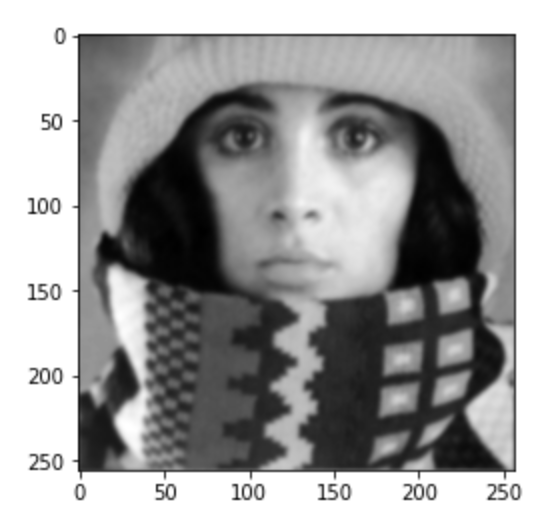
\includegraphics[width=\textwidth]{Materials/004}
		\caption{$\sigma = 0.004$.}
	\end{subfigure}
	\hfill
	\begin{subfigure}[b]{0.45\textwidth}
		\centering
		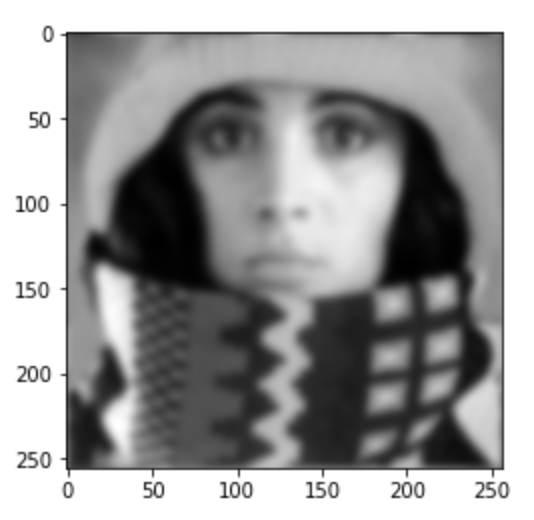
\includegraphics[width=\textwidth]{Materials/01}
		\caption{$\sigma = 0.01$.}
	\end{subfigure}
	\hfill
	\\
	\begin{subfigure}[b]{0.45\textwidth}
		\centering
		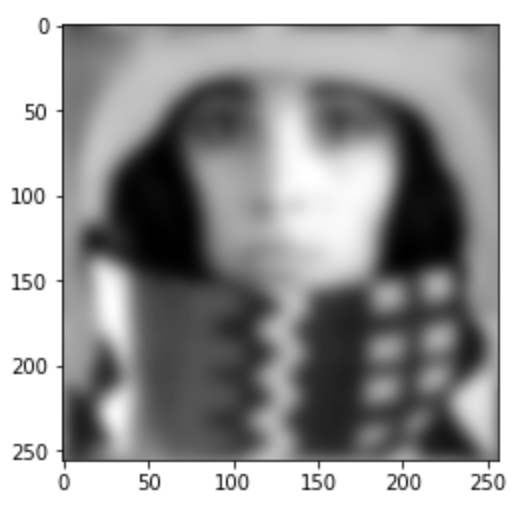
\includegraphics[width=\textwidth]{Materials/02}
		\caption{$\sigma = 0.02$.}
	\end{subfigure}
	\hfill
	\begin{subfigure}[b]{0.45\textwidth}
		\centering
		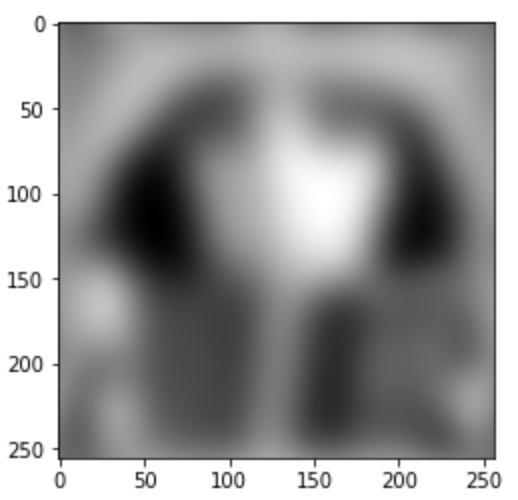
\includegraphics[width=\textwidth]{Materials/05}
		\caption{$\sigma = 0.05$.}
	\end{subfigure}
	\caption{Gaussian kernel constructed in frequency space multiplied by Fourier transform of \textit{'trui'}.}
	\label{gaussian}
\end{figure}

From the convolution theorem we know that convolution in the spatial domain is equal to multiplication in frequency domain. That is:
\begin{equation*}
		\mathcal{F}{f*g}(u) = \mathcal{F}{f}(u)\cdot \mathcal{F}{g}(u) = F(u)\cdot G(u)
\end{equation*}
Thus, if we want to perform convolution between two functions, we can instead find both functions Fourier transform, multiply these together, and then take the inverse Fourier transform of the result.\\
In \autoref{gaussian} we see the result of constructing a Gaussian kernel in frequency space and multiply it with the Fourier transform of \textit{'trui.png'} and then take the inverse Fourier transform of the result. The code used for this exercise can be seen in \autoref{e31code}. The kernel constructed by \textit{'fftgausK'} is defined based on the Fourier transform of a Gaussian kernel given in the lecture slides.
\begin{figure}[H]
	\centering
	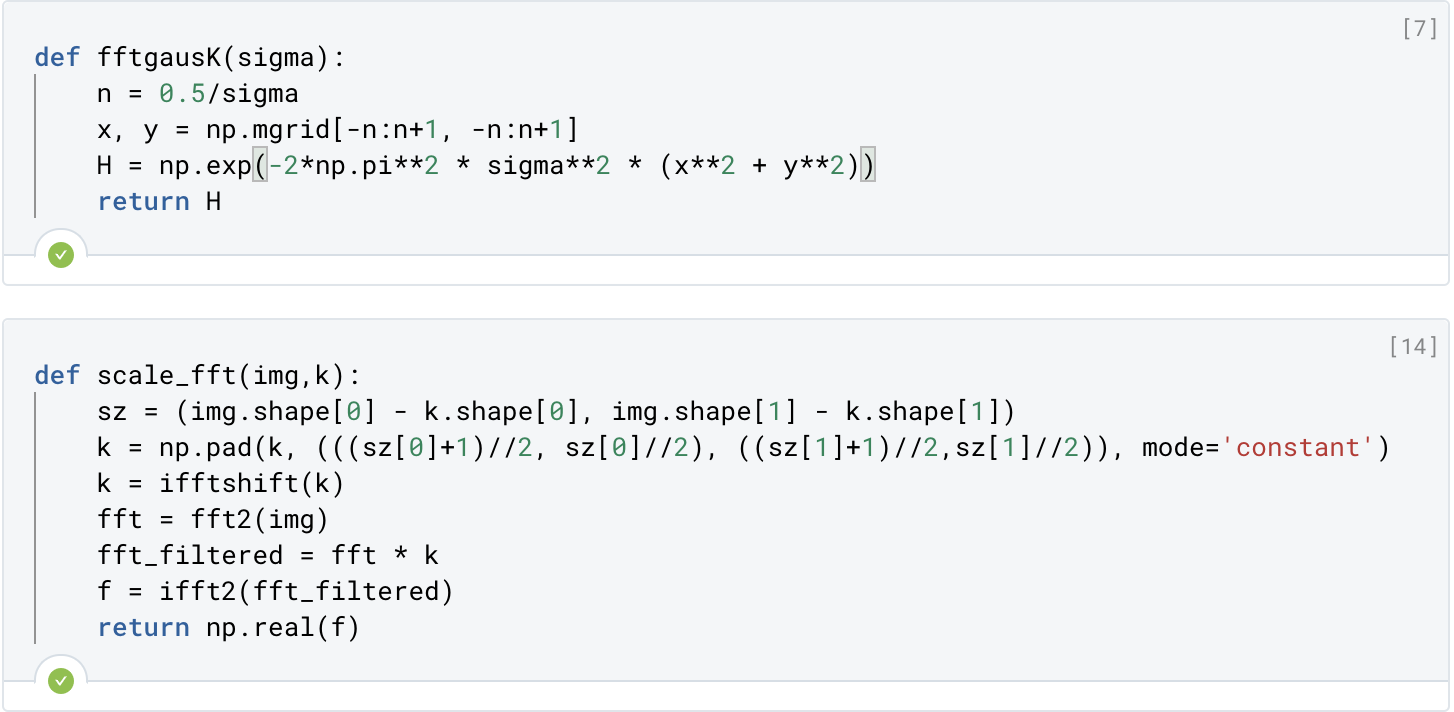
\includegraphics[width=\linewidth]{Materials/e31code}
	\caption{Code for exercise 3.1.}
	\label{e31code}
\end{figure}

\subsection*{3.2}
\begin{figure}[H]
	\centering
	\begin{subfigure}[b]{0.45\textwidth}
		\centering
		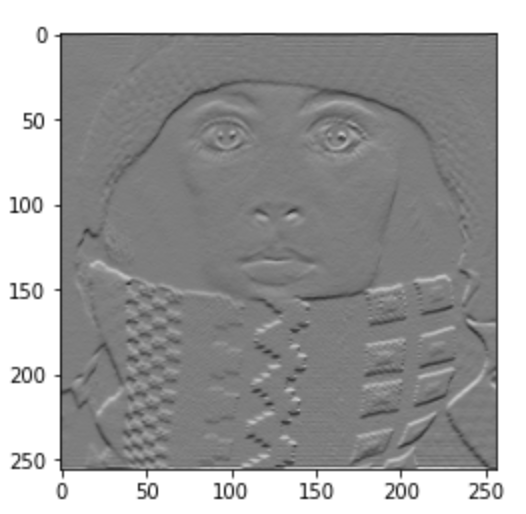
\includegraphics[width=\textwidth]{Materials/3210}
		\caption{First order y derivative.}
	\end{subfigure}
	\hfill
	\begin{subfigure}[b]{0.45\textwidth}
		\centering
		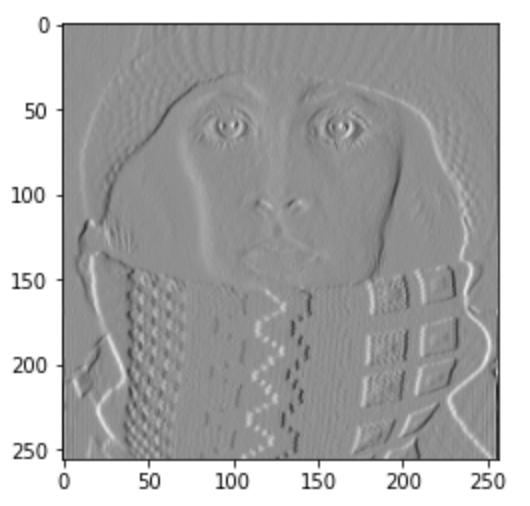
\includegraphics[width=\textwidth]{Materials/3201}
		\caption{First order x derivative.}
	\end{subfigure}
	\hfill
	\\
	\begin{subfigure}[b]{0.45\textwidth}
		\centering
		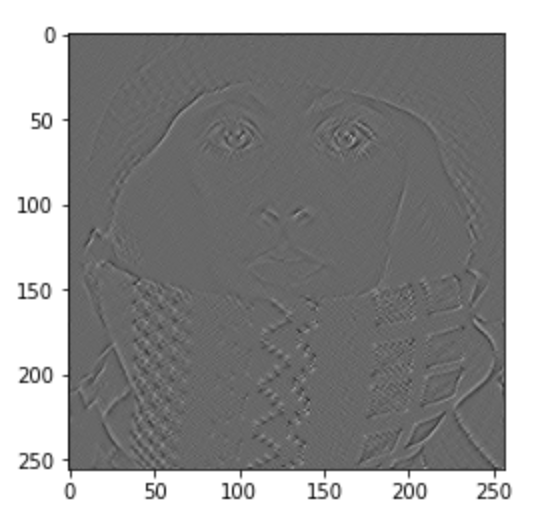
\includegraphics[width=\textwidth]{Materials/3211}
		\caption{First order x and y derivative.}
	\end{subfigure}
	\hfill
	\begin{subfigure}[b]{0.45\textwidth}
		\centering
		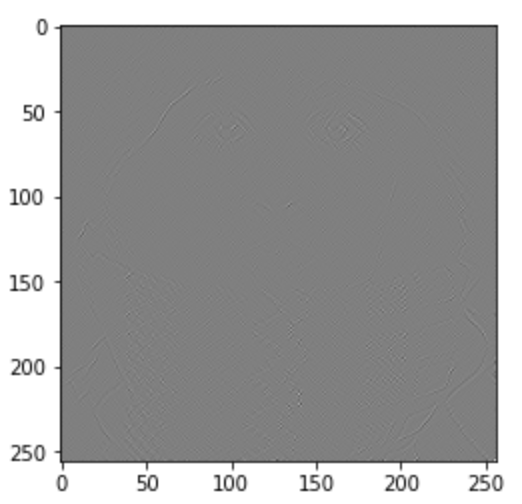
\includegraphics[width=\textwidth]{Materials/3222}
		\caption{Second order x and y derivative.}
	\end{subfigure}
	\caption{Partial derivatives of \textit{'trui'} image.}
	\label{deriv}
\end{figure}

From the lecture slides we have the derivative theorem which tells us $\frac{\partial^m}{\partial x^m}\frac{\partial^n}{\partial y^n}f(x,y)$ in spatial domain is equivalent to $(iu)^m(iv)^bF(u,v)$ in the frequency domain. That is, we can construct a kernel based on $(iu)^m(iv)^b$, multiply by $F(u,v)$ and then take the inverse Fourier transform to get our partial derivatives. The results can be seen in \autoref{deriv} and the code can be seen in \autoref{e32code}.
\begin{figure}[H]
	\centering
	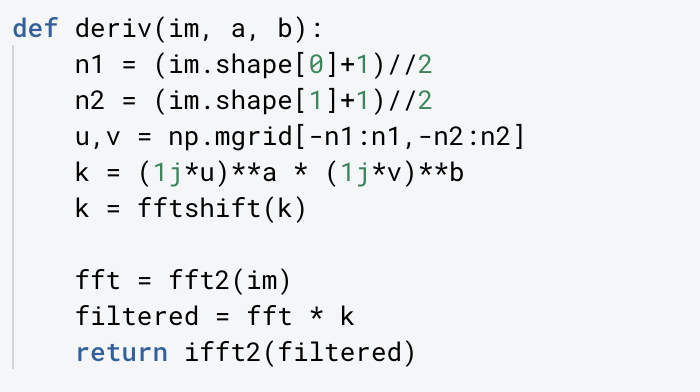
\includegraphics[width=0.7\linewidth]{Materials/e32code}
	\caption{Code for exercise 3.2.}
	\label{e32code}
\end{figure}